\documentclass[8pt]{innovativeinnovation-cheatsheet}
\definecolor{myred}{RGB}{250,127,111}
\usepackage{enumitem}
\usepackage{graphicx}
\graphicspath{{../img/}}
\newcommand{\myinline}[1]{{\color{innoinnored}\bfseries\ttfamily{#1}}}
\newtheorem{assumption}{Assumption}
\newcount\myfigurecount
\newcount\mytablecount
\myfigurecount = 1
\mytablecount = 1

\lstset{
    basicstyle=\ttfamily,
    breaklines=true,
    breakatwhitespace=true,
    tabsize=4,
    showstringspaces=true,
    extendedchars=true,
    inputencoding=utf8,
    frame=single,
    language=Matlab,
    captionpos=b,
    keywordstyle=\color{innoinnored}\bfseries,
%     numbers=left,
%     numberstyle=\tiny\color{gray},
}



\cheatsheettitle{MATLA Cheat Sheet --- Youhao HU}

\begin{document}

\begin{multicols*}{3}


\cheatsheetsection{MATLAB Command line}

\begin{enumerate}[label=$\bullet$,leftmargin=*,nosep]
    \item \lstinline!dir!: list files and folders in current folder
    \item \lstinline!dir('*.txt')!: find txt files in current folder
    \item \lstinline!pwd!: show current folder
    \item \lstinline!cd!:  change current folder
    \item \lstinline!delete('filename')!: delete file
    \item {\color{innoinnored}\bfseries\ttfamily movefile}\lstinline{('oldpath/oldname','newpath/newname')}: rename or move file    
    \item \lstinline!what!: list Matlab/simulink files in current folder
    \item {\color{innoinnored}\bfseries\ttfamily more on}: display output one screen at a time, space to continue, q to quit
    \item {\color{innoinnored}\bfseries\ttfamily more off}: display output continuously
    \item {\color{innoinnored}\bfseries\ttfamily warning off}: turn off warning
\end{enumerate}

\cheatsheetsection{Find files using Regular Expression}


\begin{enumerate}[label=$\bullet$,leftmargin=*,nosep]
    \item \myinline{dir}\verb|('*.txt')|: Find the files with extension ``txt''
    \item \myinline{dir}\verb|('*motor*')|: Find the files with ``motor'' in the file name
\end{enumerate}


\begin{center}
Table \the\mytablecount. Some rules of the regular expression
\advance\mytablecount by 1

\begin{tabular}{cp{.8\linewidth}}
\hline
Code                        & Meaning\\
\hline
\myinline{*}                & Match any characters\\
\myinline{.}                & Match any single character\\
\myinline{\textbackslash w} & Match a word character (letter/digit/underscore/Chinese character)\\
\myinline{\textbackslash s} & Match a single space\\
\myinline{\textbackslash d} & Match a single digit\\
\myinline{\textbackslash b} & Match a single word boundary (Namely the beginning/end of a word)\\
\myinline{$\hat{}$}         & Match the beginning of a line\\
\myinline{\$}               & Match the end of a line\\
\hline
\end{tabular}
\end{center}


\cheatsheetsection{Legend/title rendered in \LaTeX}

\begin{lstlisting}
h = legend(legend1,legend2);% for instance, legend1 = $x_1$
h.Interpreter = 'latex';
h.FontSize    = fontsize;
h.Location    = 'northeast';
h.Orientation = 'horizon';
title('nameoftitle','interpreter','latex')% for instance, name = $V_o$
\end{lstlisting}

\cheatsheetsection{Multi lines of title}


\begin{lstlisting}    
title({'This is the first line'; 'This is the second line'});
\end{lstlisting}

\cheatsheetsection{Save figure}


\begin{lstlisting}
saveas(gcf,'filename','png'); % No resolution ratio option
print(gcf,'-dpng', '-r300', 'filename'); % 300 dpi png
\end{lstlisting}

\cheatsheetsection{Data interpolation / Prediction of missing data}

Match the data \myinline{iL1out} with the simulation time vector \myinline{toutSIM}.
\begin{enumerate}[label=$\bullet$,leftmargin=*,nosep]
    \item Original data: \myinline{(t,iL1out)}
    \item New data: \myinline{(toutSIM,iL1out)}
\end{enumerate}

\begin{lstlisting}
iL1out = interp1(t,iL1out,toutSIM)
\end{lstlisting}


\begin{enumerate}[label=$\bullet$,leftmargin=*,nosep]
    \item Original data: \myinline{(t,iL1out)}
    \item Wanted point: \myinline{(t1,iL1)}
\end{enumerate}

\begin{lstlisting}
iL1 = interp1(t,iL1out,t1)
\end{lstlisting}


\cheatsheetsection{The greatest common divisor / The least common multiple}

\begin{enumerate}[label=$\bullet$,leftmargin=*,nosep]
    \item \lstinline!gcd(a,b)!: The greatest common divisor of a and b 
    \item \lstinline!lcm(a,b)!: The least common multiple of a and b
\end{enumerate}

\cheatsheetsection{GA to tune parameters in Simulink}
\begin{lstlisting}
clc,clear,close all

SimulinkModel = 'DCMotorPID'; % Simulink model name, case-insensitive.
open(SimulinkModel);
fun = @GATestFun;
nvars = 4;
lb = [0;0;0;20000];
ub = [.1;.1;.1;40000];
MaxGen  = 1;
PopSize = 10; % Large size brings better result, but takes more time.
options = optimoptions('ga', 'PopulationSize', PopSize, 'MaxGenerations', MaxGen, 'Display', 'iter');
[x,fval,exitflag] = ga(fun, nvars, [], [], [], [], lb, ub, [], options);


%------------------------------------------
%--- Display the parameters tuned by GA ---
%------------------------------------------

kp = x(1)
ki = x(2)
kd = x(3)
fN = x(4)


%------------------------------------------
%--- Show the result ---
%------------------------------------------

hws = get_param(SimulinkModel,'modelworkspace');
hws.assignin('kp',kp);
hws.assignin('ki',ki);
hws.assignin('kd',kd);
hws.assignin('fN',fN);

simout = sim(SimulinkModel);

t          = simout.simout.Time;
SpeedError = simout.simout.Data;
plot(t,SpeedError,'LineWidth',1.5)
title('$Tracking Error$','interpreter','latex')
grid on

%-----------------------------------------------
%--- The cost function to evaluate the error ---
%-----------------------------------------------

function cost = GATestFun(inputpara)

SimulinkModel = 'DCMotorPID';
kp = inputpara(1);
ki = inputpara(2);
kd = inputpara(3);
fN = inputpara(4);

hws = get_param(SimulinkModel, 'modelworkspace');
hws.assignin('kp',kp)
hws.assignin('ki',ki)
hws.assignin('kd',kd)
hws.assignin('fN',fN)
simout = sim(SimulinkModel);
cost   = rms(simout);
end
\end{lstlisting}


\begin{center}
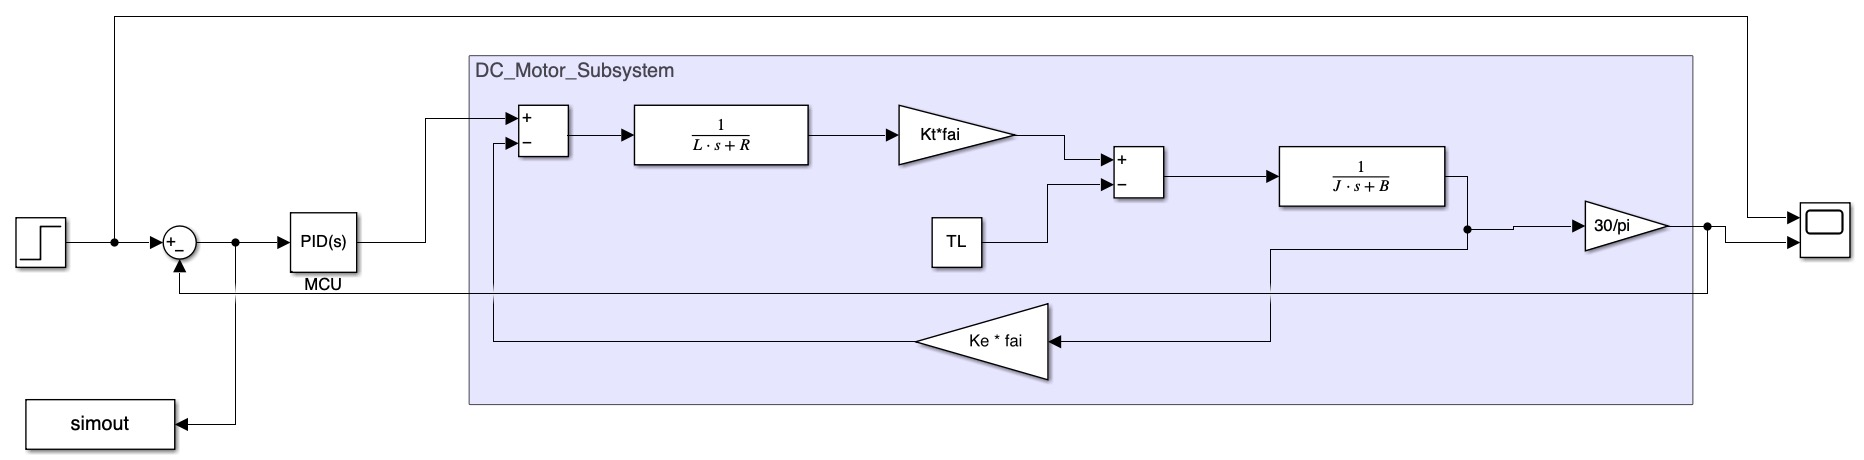
\includegraphics[width = \linewidth]{DCMotorSimulinkModel}
Figure 1. Simulink Model
\end{center}

\begin{center}
Table 1. Parameters in the Simulink Model
\begin{tabular}{cc||cc}
\hline
Parameters & Values & Parameters & Values\\
\hline
\myinline{Ke} & 0.1                     & \myinline{fai} & 0.1\\
\myinline{Kt} & \myinline{Ke} * 30 / pi & \myinline{J}   & 0.001\\
\myinline{L}  & 0.005                   & \myinline{B}   & 0.01 \\
\myinline{R}  & 0.1                     & \myinline{TL}  & 0\\
\hline
\end{tabular}
\end{center}


\cheatsheetsection{Resample the data}

Suppose there is a data set $(t,V_{RL})$ obtained from SIMULINK, we want to resample it to reduce the data size:

\begin{lstlisting}
told   = simuout.out.simout.Time;
VRLold = simuout.out.simout.Data(:,1);

dtold  = mean(diff(t)); % Original sampling time
dtnew  = .2e-3;         % New even sampling time
Q      = round(dtnew/dtold); % Resample rate
tnew   = t(1):dtnew:length(VRL);
VRLnew = resample(simuout.out.simout.Data(:,1),1,Q);

\end{lstlisting}

\cheatsheetsection{Solve function}


\begin{lstlisting}
syms x
eq = x^2 == 1;
solve(eq,x)
\end{lstlisting}


\cheatsheetsection{Solve function numerically}


\begin{lstlisting}
syms x
eq = sin(x)^2 == 1;
vpasolve(eq,x,5) % 5 digits, default is 32 digitss
\end{lstlisting}

\cheatsheetsection{Symbol value to numemrical value}


\begin{lstlisting}
syms x
solSym = solve(x^2 == 1,x)
solNum = vpa(solSym,5) % 5 digits, default is 32 digits
\end{lstlisting}

\cheatsheetsection{Subsitute value into symbolic expression}


\begin{lstlisting}
syms x
subs(x^2,x,2)
\end{lstlisting}

\cheatsheetsection{Symbolic to double}


\begin{lstlisting}
syms x
SymVar = int(x^2,x,0,1);
VpaVar = vpa(SymVar,5); % 5 digits, default is 32 digits
DblVar = double(VpaVar);
\end{lstlisting}

\cheatsheetsection{Polynomial fit}


\begin{lstlisting}
x = 0:0.1:.5;
y = sin(x);
p = polyfit(x,y,1); % 1st order polynomial fit

plot(x,y)
hold on
plot(x,p(1) * x + p(2))
\end{lstlisting}

\cheatsheetsection{Troubleshooting}

Q: SIMULINK does not work properly even with identical parameters.

A: Check the workspace priority, 
making sure variables are well defined and 
no other higher priority variables with the same name.
\begin{itemize}
    \item \myinline{Higher priority:} Model workspace.
    \item \myinline{Lower priority:} Base workspace.
\end{itemize}






\vfill

\cheatsheetfooter{Innovative Innovation}{https://github.com/innovativeinnovation}

\end{multicols*}

\end{document}
